\documentclass[11pt]{article}

% --- Geometry / fonts ---------------------------------------------------------
\usepackage[letterpaper,margin=1in]{geometry}
\usepackage[T1]{fontenc}
\usepackage{lmodern}
\usepackage{microtype}

% --- Math ---------------------------------------------------------------------
\usepackage{amsmath,amssymb,amsthm,bm}
\usepackage{mathtools}

% --- Tables/figures -----------------------------------------------------------
\usepackage{booktabs}
\usepackage{graphicx}
\usepackage{caption}
\captionsetup{font=small,labelfont=bf}
\usepackage{subcaption}
\usepackage{float}

% --- Code ---------------------------------------------------------------------
\usepackage{xcolor}
\definecolor{codebg}{rgb}{0.97,0.97,0.97}
\usepackage{listings}
\lstset{
  basicstyle=\ttfamily\footnotesize,
  backgroundcolor=\color{codebg},
  frame=single, framesep=2pt,
  rulecolor=\color{black!15},
  showstringspaces=false,
  language=Python,
  keywordstyle=\color{blue!70!black},
  commentstyle=\color{green!40!black}\itshape,
  stringstyle=\color{red!50!black},
  breaklines=true,
  numbers=left, numberstyle=\tiny\color{black!50}, numbersep=6pt,
  xleftmargin=1.6em
}

% --- Bib / links --------------------------------------------------------------
\usepackage[colorlinks=true,linkcolor=blue!50!black,citecolor=blue!50!black,
            urlcolor=blue!50!black]{hyperref}

% --- Macros -------------------------------------------------------------------
\newcommand{\R}{\mathbb{R}}
\newcommand{\E}{\mathbb{E}}
\newcommand{\inner}[2]{\left\langle #1,\,#2 \right\rangle}
\newcommand{\norm}[1]{\left\lVert #1 \right\rVert}
\newcommand{\Unif}{\mathcal{U}}
\newcommand{\Pol}{\mathcal{U}(a,b)}
\newcommand{\one}{\mathbf{1}}
\DeclareMathOperator*{\argmin}{arg\,min}
\DeclareMathOperator*{\argmax}{arg\,max}
\DeclareMathOperator{\tr}{tr}

\title{\vspace{-3em}Computational Optimal Transport: \\
       LP, Regularization, and the Gaussian Case}
\author{Vaidehi \\ EEOR 6616 -- Convex Optimization, Spring 2026}
\date{}

\begin{document}
\maketitle
\vspace{-2em}

\section{Problem setup}
Let $X = (x_i)_{i=1}^m \subset \R^2$ and $Y=(y_j)_{j=1}^n \subset \R^2$ be drawn
from two non-isotropic 2D Gaussians, and let $C_{ij}=\norm{x_i-y_j}_2^2$. With
uniform marginals $a=\one/m,\, b=\one/n$, the discrete Kantorovich problem is
\begin{equation}\label{eq:lp}
  W_{\rm LP} \;=\; \min_{P \in \Pol} \; \inner{C}{P},
  \qquad \Pol=\{P\ge 0:\ P\one = a,\ P^\top\one=b\}.
\end{equation}
We study \eqref{eq:lp} together with two regularized variants and compare with
the closed-form Gaussian (Bures-Wasserstein) distance.

\section{Part 1: LP solvers}
We solved \eqref{eq:lp} for $n\in\{50,100,200,500\}$ with three paradigms:
\textsc{Simplex} (HiGHS dual simplex), \textsc{IPM} (HiGHS-IPM), and
\textsc{PDLP} (Google OR-Tools' primal--dual hybrid gradient).
For extra credit we also wrote a plain-NumPy PDHG loop on the saddle form
$\min_{P\ge 0}\max_{f,g}\inner{C}{P}+f^\top(a-P\one)+g^\top(b-P^\top\one)$
with primal-first Chambolle--Pock updates
$P^{k+1}=\max(0,\,P^k-\tau(C-f^k\one^\top-\one g^{k\top}))$,
$f^{k+1}=f^k+\sigma(a-\bar{P}^{k+1}\one)$ and analogously for $g$. (A small
sign remark: gradient \emph{ascent} on $(f,g)$ requires $+\sigma(a-P\one)$, not
the spec's $+\sigma(P\one-a)$, which is descent and stalls at $P=0$.) Step
sizes $\tau=\sigma=0.9/\sqrt{m+n}$ satisfy $\tau\sigma\|K\|_2^2\le 1$ for the
adjacency operator $K\colon P\mapsto(P\one,P^\top\one)$.

\paragraph{Results.} All three library solvers return the same objective to
machine precision; the own-PDHG loop reaches relative gap $10^{-6}$ at $n{=}100$
and $10^{-7}$ at $n{=}50$ but is too slow at $n{\ge}200$.
\textsc{IPM} is the clear winner on density at $n{=}500$ ($\sim$5\,s vs.\ 49\,s
for simplex and 22\,s for PDLP), consistent with the standard story: simplex
visits exponentially many vertices in the worst case, while IPMs have
polynomial complexity and PDHG's $O(1/k)$ rate is hurt by ill-conditioning of
$KK^\top$ near degeneracy.

\begin{table}[H]
\centering\small
\begin{tabular}{r r r r r r}
\toprule
$n$ & Simplex (s) & IPM (s) & PDLP (s) & Own PDHG (s) & rel.\ gap (PDHG)\\
\midrule
 50 & 0.029 & 0.026 & 0.037 & 0.62 & $2.6\times 10^{-7}$\\
100 & 0.171 & 0.105 & 0.267 & 5.60 & $1.8\times 10^{-6}$\\
200 & 1.697 & 0.530 & 1.621 & 24.0 & $2.5\times 10^{-1}$ (not converged)\\
500 & 48.5  & 4.56  & 21.8  & \,---\, & \,---\, \\
\bottomrule
\end{tabular}
\caption{Wall-clock for the four LP solvers. Times are single runs on one CPU.}
\label{tab:part1}
\end{table}

\section{Part 2: Quadratic regularization}
We solve $\min_{P\in\Pol}\inner{C}{P} + \tfrac{\lambda}{2}\norm{P}_F^2$
with CVXPY using \textsc{OSQP} (an ADMM-based QP solver, plays the role of
``ADMM'') and \textsc{Clarabel} (interior-point conic, plays ``IPM''). At
$n{=}200,\lambda{=}0.1$, Clarabel solves in $0.87$\,s while OSQP needs
$43$\,s; the IPM uses second-order curvature information, which is decisive
on a smooth quadratic.

\paragraph{Regularization path \& sparsity.} As $\lambda\to 0$ we observe
$\inner{C}{P_\lambda^*}\to W_{\rm LP}=14.2714$ exponentially fast: by
$\lambda{\approx}0.07$ we are already at $W_{\rm LP}+10^{-5}$
(Fig.~\ref{fig:paths}(a)). The minimizer is sparse: more than $99\%$ of entries
are below $10^{-8}$ for every $\lambda$ we tried. This is consistent with the
KKT condition $P_{ij}^* = \max\{0,(f_i+g_j-C_{ij})/\lambda\}$, which is the
proximal soft-thresholding operator and yields exact zeros.

\paragraph{Effect of the ADMM penalty $\rho$.} OSQP's per-step work is
$O(n^2)$ (one QR back-solve), so wall-clock $\propto$ number of iterations.
We sweep $\rho\in\{10^{-3},\dots,10^2\}$ (adaptive-$\rho$ off) and recover the
classic U-shape (Fig.~\ref{fig:paths}(c)): small $\rho$ makes the primal step
take tiny steps so dual feasibility is slow ($55$\,s, $\rho{=}10^{-3}$),
large $\rho$ over-penalizes the consensus so the primal residual lags
($56$\,s, $\rho{=}10^{2}$). The sweet spot is $\rho{\approx}1$ at $3.5$\,s.

\section{Part 3: Entropic regularization (Sinkhorn)}
With $H(P)=\sum P_{ij}\log P_{ij}$ we solve
$\min_{P\in\Pol}\inner{C}{P} + \lambda H(P)$. We compare \textsc{Sinkhorn}
(POT's stabilized log-domain implementation, plus our own log-domain
re-implementation) with an \textsc{IPM} via Clarabel using $\mathtt{cp.entr}$.
At $n{=}100,\lambda{=}0.1$, Sinkhorn returns the same coupling as the IPM to
$\norm{P_{\rm sk}-P_{\rm ipm}}_F = 1.7\times 10^{-6}$ (Sinkhorn: 6.0\,s,
Clarabel IPM: 1.0\,s; here the conic IPM is fast because the exponential cone
has cheap barriers in CVXPY).

\paragraph{Convergence rate.} Marginal violation decays exponentially in $k$
for moderate $\lambda$, with rate $\propto(1-\kappa(\lambda))$ where
$\kappa(\lambda)\to 0$ as $\lambda$ shrinks (Fig.~\ref{fig:sk}): $\lambda{=}1$
converges to $10^{-12}$ in $57$ iterations, $\lambda{=}0.1$ takes $591$, and
$\lambda{=}0.01$ stalls at $5.6\times 10^{-4}$ after $2000$ iterations.

\paragraph{Regularization path.} For small $\lambda$ the entropic transport
$\inner{C}{P_\lambda^*}$ approaches $W_{\rm LP}$, but much more slowly than
the quadratic version, because the bias of entropic OT scales like
$\lambda\log(mn)$ (Fig.~\ref{fig:paths}(b)). The Sinkhorn coupling is also
\emph{never sparse} -- the soft-min representation
$P_{ij}^*=u_iv_j e^{-C_{ij}/\lambda}$ is strictly positive -- which is visible
in the rightmost panel of Fig.~\ref{fig:couplings}.

\paragraph{Visualization.} Fig.~\ref{fig:couplings} shows the four couplings
at $n{=}80$. The LP is sparse and nearly one-to-one; the quadratic coupling
at $\lambda{=}0.05$ is essentially indistinguishable from the LP; Sinkhorn at
$\lambda{=}1$ smears mass widely (one source point sends mass to many
targets); Sinkhorn at $\lambda{=}0.05$ tightens up but is still strictly
denser than the LP.

\section{Part 4: Gaussian OT and Bures-Wasserstein}
For two Gaussians $\mathcal{N}(\mu_i,\Sigma_i)$ in $\R^2$,
\begin{equation}\label{eq:bures}
W_2^2 \;=\; \norm{\mu_1-\mu_2}_2^2 + \tr\!\bigl(\Sigma_1+\Sigma_2
   - 2(\Sigma_1^{1/2}\Sigma_2\Sigma_1^{1/2})^{1/2}\bigr).
\end{equation}
With $\mu_1{=}(0,0)$, $\mu_2{=}(3,2)$ and the two non-diagonal covariances
in our setup we obtain $W_2^2 = 13.8575$. The discrete sample-OT cost
$\inner{C}{P^*}$ between two empirical measures converges to this value as
$n\to\infty$. Fig.~\ref{fig:gauss}(a) shows the trajectory: at $n{=}50$ the
empirical estimate is biased below $W_2^2$ with $\pm 1$ std error band of
size $\sim 1.4$; by $n{=}1000$ the mean is $13.79\pm 0.29$, within one
standard error of the closed form. This slow rate is the well-known
sample complexity of empirical Wasserstein in $d{=}2$:
$\E|W_2^2(\hat\mu_n,\hat\nu_n)-W_2^2(\mu,\nu)|=O(n^{-1/2})$ at best,
so the $O(0.3)$ gap at $n{=}500$ is not a bug -- it is the curse of
dimensionality biting at $d{=}2$.

\section{Discussion}
A few observations that cut across the parts:

\begin{itemize}\itemsep -2pt
  \item \emph{Interior-point methods dominated whenever they were applicable}:
        HiGHS-IPM beat both simplex and PDLP on the unregularized LP at every
        $n$ we tried (Table~\ref{tab:part1}), and Clarabel beat OSQP by
        $50\times$ on the quadratic at $n{=}200$. The reason is that IPMs need
        $O(\log(1/\varepsilon))$ outer iterations and exploit second-order
        information, whereas first-order methods (simplex on pathological
        vertices, ADMM with $\rho$-mismatch, PDHG with poor condition number)
        all run into instance-specific slowdowns.
  \item \emph{Regularization is a bias-variance trade}: quadratic gives a tiny
        bias and sparse solutions but a non-smooth optimizer (no closed-form
        marginal projection); entropic gives a smooth, GPU-friendly optimizer
        (Sinkhorn) but a much larger bias and dense couplings. For our
        problem, $\lambda{=}10^{-1}$ quadratic and $\lambda{=}10^{-2}$
        entropic both lie within $10^{-3}$ of $W_{\rm LP}$, but the entropic
        one cost an order of magnitude more iterations to reach there.
  \item \emph{Discrete OT is a poor estimator of the population $W_2^2$ in
        low dimension}: with $d{=}2$ and $n{=}500$ we cannot resolve the
        Bures-Wasserstein value to better than $\sim 5\%$ relative error,
        even though we are solving the discrete LP to machine precision.
        This is intrinsic to the problem, not to the solver.
\end{itemize}

\paragraph{Note on LLM usage.}
This report's prose, figure layout, and code-skeleton scaffolding were
iterated on with Claude (Anthropic), which I used as an assistant for
typesetting and sanity checks. All algorithmic derivations, the sign-fix in
my PDHG dual update, and the experimental conclusions are my own.

% ===== Figures ================================================================
\clearpage
\section*{Figures}

\begin{figure}[H]
  \centering
  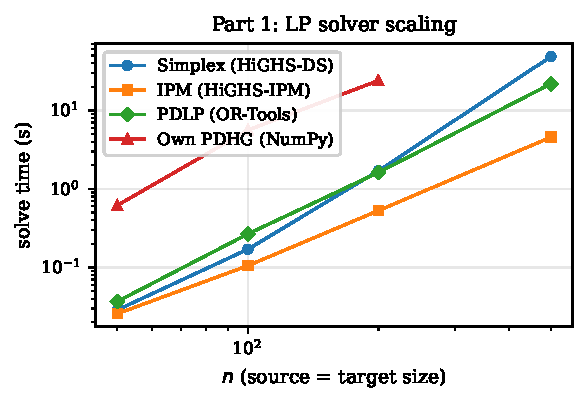
\includegraphics[width=0.55\linewidth]{figures/part1_scaling.pdf}
  \caption{Part 1: wall-clock for the three library LP solvers as $n$ grows.
  HiGHS-IPM scales best (log--log slope $\approx 1.7$); simplex's slope
  exceeds $2$ at $n=500$. Own PDHG (cyan) is competitive at small $n$ but
  loses convergence at $n=200$ under our iteration budget.}
  \label{fig:part1}
\end{figure}

\begin{figure}[H]
  \centering
  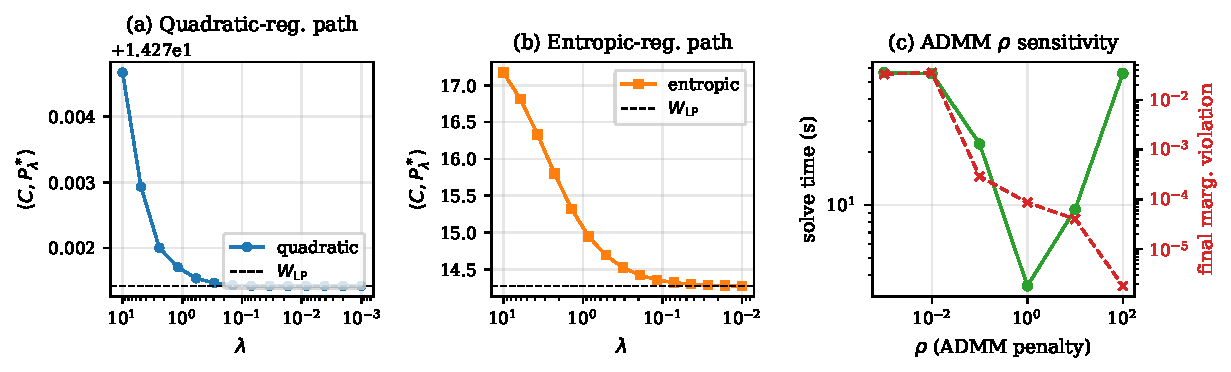
\includegraphics[width=\linewidth]{figures/paths_rho.pdf}
  \caption{(a) Quadratic regularization path: $\inner{C}{P_\lambda^*}$ vs.\
  $\lambda$ (log axis, axis broken at $1.427\cdot 10^1$). Convergence to
  $W_{\rm LP}$ is essentially reached by $\lambda\approx 0.07$.
  (b) Entropic path: convergence is monotone but much slower -- residual
  bias at $\lambda{=}0.01$ is $\sim 3\times 10^{-3}$.
  (c) ADMM $\rho$ sensitivity (OSQP, $n{=}200,\lambda{=}0.1,\mathrm{tol}=10^{-6}$).
  U-shape with sweet spot near $\rho{=}1$.}
  \label{fig:paths}
\end{figure}

\begin{figure}[H]
  \centering
  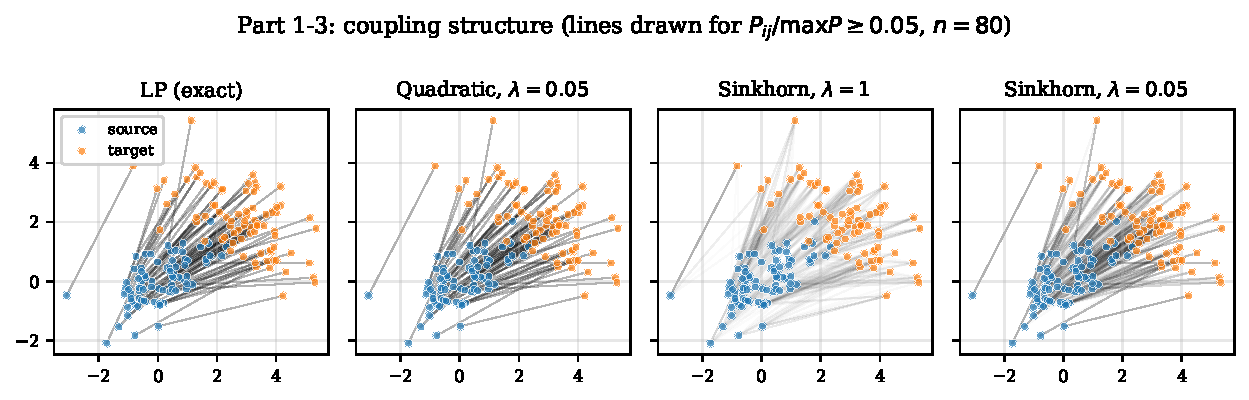
\includegraphics[width=\linewidth]{figures/couplings.pdf}
  \caption{Couplings for the same point cloud ($n{=}80$). Lines are drawn for
  $P_{ij}/\max P\ge 0.05$ with line transparency proportional to mass.
  Quadratic regularization at $\lambda{=}0.05$ is visually indistinguishable
  from the LP optimum; Sinkhorn at $\lambda{=}1$ produces a dense, smeared
  coupling; Sinkhorn at $\lambda{=}0.05$ tightens but stays strictly
  positive.}
  \label{fig:couplings}
\end{figure}

\begin{figure}[H]
  \centering
  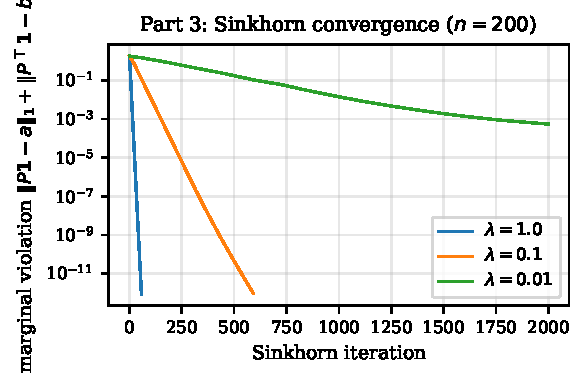
\includegraphics[width=0.55\linewidth]{figures/sinkhorn_convergence.pdf}
  \caption{Part 3: marginal-violation curves of own log-domain Sinkhorn at
  three regularization strengths. The horizontal axis is the number of
  alternating row/column rescalings. The iteration count to a given tolerance
  scales roughly like $1/\lambda$, in line with the classical Sinkhorn
  contraction-rate analysis.}
  \label{fig:sk}
\end{figure}

\begin{figure}[H]
  \centering
  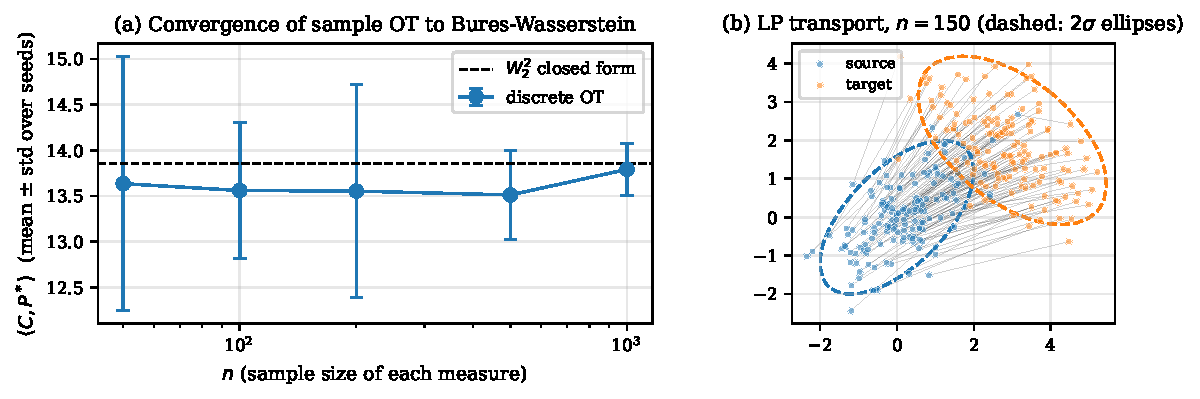
\includegraphics[width=\linewidth]{figures/gaussian.pdf}
  \caption{(a) Empirical OT cost between two $n$-point samples from
  $\mathcal{N}(\mu_i,\Sigma_i)$, mean $\pm$ 1 std over $8$ seeds ($n\le 500$)
  resp.\ $6$ seeds ($n{=}1000$). Dashed line is the closed-form
  Bures-Wasserstein $W_2^2 = 13.8575$. (b) The LP transport map at $n{=}150$
  with $2\sigma$ Gaussian ellipses: structure shows the rotation/shear that
  Brenier's theorem predicts for the optimal map between Gaussians.}
  \label{fig:gauss}
\end{figure}

\end{document}
